%%%%%%%%%%%%%%%%%%%%%%%%%%%%%%%%%%%%%%%%%%%%%%%%%%%%%%%%%%%%%%%%%%%%%%%%%%%%%%%%
\subsection{Brief background for derivation of the cable equation}
%%%%%%%%%%%%%%%%%%%%%%%%%%%%%%%%%%%%%%%%%%%%%%%%%%%%%%%%%%%%%%%%%%%%%%%%%%%%%%%%
See \cite{lindsay_2004} for a detailed derivation of the cable equation, and extensions to the one-dimensional model that account for radial variation of potential.

The one-dimensional cable equation introduced later in equations~\eq{eq:cable} and~\eq{eq:cable_balance} is based on the following expression in three dimensions (based on Maxwell's equations adapted for neurological modelling)
\begin{equation}
    \nabla \cdot \vv{J} = 0,
    \label{eq:J}
\end{equation}
where $\vv{J}$ is current density (units $A/m^2$).
Current density is in turn defined in terms of electric field $\vv{E}$ (units $V/m$)
\begin{equation}
    \vv{J} = \sigma \vv{E},
\end{equation}
where $\sigma$ is the specific electrical conductivity of intra-cellular fluid (typically 3.3 $S/m$).

The derivation of the cable equation is based on two assumptions:
\begin{enumerate}
    \item that charge disperion is effectively instantaneous for the purposes of dendritic modelling.
    \item that diffusion of magnetic field is instant, i.e. it behaves quasi-statically in the sense that it is determined by the electric field through the Maxwell equations.
\end{enumerate}
Under these conditions, $\vv{E}$ is conservative, and as such can be expressed in terms of a potential field
\begin{equation}
    \vv{E} = \nabla \phi,
\end{equation}
where the extra/intra-cellular potential field $\phi$ has units $mV$.

The derivation of the one-dimensional conservation equation \eq{eq:cable_balance} is based on the assumption that the intra-cellular potential (i.e. inside the cell) does not vary radially.
That is, potential is a function of the axial distance $x$ alone
\begin{equation}
    \vv{E} = \nabla \phi = \pder{V}{x}.
\end{equation}
This is not strictly true, because a potential field that is a variable of $x$ and $t$ alone can't support the axial gradients required to drive the potential difference over the cell membrane.
I am still trying to get my head around the assumptions made in mapping a three-dimensional problem to a pseudo one-dimensional one.

%%%%%%%%%%%%%%%%%%%%%%%%%%%%%%%%%%%%%%%%%%%%%%%%%%%%%%%%%%%%%%%%%%%%%%%%%%%%%%%%
\subsection{The cable equation}
%%%%%%%%%%%%%%%%%%%%%%%%%%%%%%%%%%%%%%%%%%%%%%%%%%%%%%%%%%%%%%%%%%%%%%%%%%%%%%%%
The cable equation is a nonlinear parabolic PDE that can be written in the form
\begin{equation}
    \label{eq:cable}
    c_m \pder{V}{t} = \frac{1}{2\pi a r_{L}} \pder{}{x} \left( a^2 \pder{V}{x} \right) - i_m + i_e,
\end{equation}
where
\begin{itemize}
    \item $V$ is the potential relative to the ECM $[mV]$
    \item $a$ is the cable radius $(mm)$, and can vary with $x$
    \item $c_m$ is the {specific membrane capacitance}, approximately the same for all neurons $\approx 10~nF/mm^2$. Related to \emph{membrane capacitance} $C_m$ by the relationship $C_m=c_{m}A$, where $A$ is the surface area of the cell.
    \item $i_m$ is the membrane current $[A\cdot/mm^{2}]$ per unit area. The total contribution from ion and synaptic channels is expressed as a the product of current per unit area $i_m$ and the surface area.
    \item $i_e$ is the electrode current flowing into the cell, divided by surface area, i.e. $i_e=I_e/A$.
    \item $r_L$ is intracellular resistivity, typical value $1~k\Omega \text{cm}$
\end{itemize}

Note that the standard convention is followed, whereby membrane and synapse currents ($i_m$) are positive when outward, and electrod currents ($i_e$) are positive inward.

The PDE in (\ref{eq:cable}) is derived by integrating~\eq{eq:J} over the volume of segment $i$:
\begin{equation*}
    \int_{\Omega_i}{\nabla \cdot \vv{J} } \deriv{v} = 0,
\end{equation*}
Then applying the divergence theorem to turn the volume integral on the lhs into a surface integral
\begin{equation}
          \sum_{j\in\mathcal{N}_i} {\int_{\Gamma_{i,j}} J_{i,j} \deriv{s} }
        + \int_{\Gamma_{i}} {J_m} \deriv{s} = 0
    \label{eq:cable_balance_intermediate}
\end{equation}
where
\begin{itemize}
    \item $\int_\Omega \cdot \deriv{v}$ is shorthand for the volume integral over the segment $\Omega_i$
    \item $\int_\Gamma \cdot \deriv{s}$ is shorthand for the surface integral over the surface $\Gamma$
    \item $J_{i,j}=-\frac{1}{r_L}\pder{V}{x} n_{i,j}$ is the flux per unit area of current \emph{from segment $i$ to segment $j$} over the interface $\Gamma_{i,j}$ between the two segments.
    \item the set $\mathcal{N}_i$ is the set of segments that are neighbours of $\Omega_i$
\end{itemize}
The transmembrane current density $J_m=\vv{J}\cdot\vv{n}$ is a function of the membrane potential
\begin{equation}
    J_m = c_m\pder{V}{t} + i_m - i_e,
    \label{eq:Jm}
\end{equation}
which has contributions from the ion channels and synapses ($i_m$), electrodes ($i_e$) and capacitive current due to polarization of the membrane whose bi-layer lipid structure causes it to behave locally like a parallel plate capacitor.

Substituting~\eq{eq:Jm} into~\eq{eq:cable_balance_intermediate} and rearanging gives
\begin{equation}
      \int_{\Gamma_{i}} {c_m\pder{V}{t}} \deriv{s}
    = - \sum_{j\in\mathcal{N}_i} {\int_{\Gamma_{i,j}} J_{i,j} \deriv{s} }
    - \int_{\Gamma_{i}} {(i_m - i_e)} \deriv{s}
    \label{eq:cable_balance}
\end{equation}


The surface of the cable segment is sub-divided into the internal and external surfaces.
The external surface $\Gamma_{i}$ is the cell membrane at the interface between the extra-cellular and intra-cellular regions.
The current, which is the conserved quantity in our conservation law, over the surface is composed of the synapse and ion channel contributions.
This is derived from a thin film approximation to the cell membrane, whereby the membrane is treated as an infinitesimally thin interface between the intra and extra cellular regions.

Note that some information is lost when going from a three-dimensional description of a neuron to a system of branching one-dimensional cable segments.
If the cell is represented by cylinders or frustrums\footnote{a frustrum is a truncated cone, where the truncation plane is parallel to the base of the cone.}, the three-dimensional values for volume and surface area at branch points can't be retrieved from the one-dimensional description.

\begin{figure}
    \begin{center}
        \includegraphics[width=0.5\textwidth]{./images/cable.pdf}
    \end{center}
    \caption{A single segment, or control volume, on an unbranching dendrite.}
    \label{fig:segment}
\end{figure}

%%%%%%%%%%%%%%%%%%%%%%%%%%%%%%%%%%%%%%%%%%%%%%%%%%%%%%%%%%%%%%%%%%%%%%%%%%%%%%%%
\subsection{Finite volume discretization}
%%%%%%%%%%%%%%%%%%%%%%%%%%%%%%%%%%%%%%%%%%%%%%%%%%%%%%%%%%%%%%%%%%%%%%%%%%%%%%%%
The finite volume method is a natural choice for the solution of the conservation law in~\eq{eq:cable_balance}.

\begin{itemize}
    \item   the $x_i$ are spaced uniformly with distance $x_{i+1}-x_{i} = \Delta x$
    \item   control volumes are formed by locating the boundaries between adjacent points at $(x_{i+1}+x_{i})/2$
    \item   this discretization differs from the finite differences used in Neuron because the equation is explicitly solved for at the end of cable segments, and because the finite volume discretization is applied to all points. Neuron uses special algebraic \emph{zero area} formulation for nodes at branch points.
\end{itemize}

%-------------------------------------------------------------------------------
\subsubsection{Temporal derivative}
%-------------------------------------------------------------------------------
The integral on the lhs of~\eq{eq:cable_balance} can be approximated by assuming that the average transmembrane potential $V$ in $\Omega_i$ is equal to the potential $V_i$ defined at the centre of the segment:
\begin{equation}
    \int_{\Gamma_i}{c_m \pder{V}{t} } \deriv{v} \approx \sigma_i \cmi \pder{V_i}{t},
    \label{eq:dvdt}
\end{equation}
where $\sigma_i$ is the surface area, and $\cmi$ is the average specific membrane capacitance, respectively of the surface $\Gamma_i$.

Each control volume is composed of \emph{sub control volumes}, which are illustrated as the coloured sub-regions in \fig{fig:segment}.
\begin{equation*}
    \Omega_i = \bigcup_{j\in\mathcal{N}_i}{\Omega_i^j}.
\end{equation*}
Likewise, the surface $\Gamma_i$ is composed of subsufaces as follows
\begin{equation*}
    \Gamma_i = \bigcup_{j\in\mathcal{N}_i}{\Gamma_i^j},
\end{equation*}
where $\Gamma_i^j$ is the surface of each of the sub-control volumes in $\Omega_i$.
Thus, the surface area of the CV as
\begin{equation*}
    \sigma_i = \sum_{i\in\mathcal{N}_i}{\sigma_i^j},
\end{equation*}
where $\sigma_i^j$ is the area of $\Gamma_i^j$, and the average specific membrane capacitance $\cmi$ is
\begin{equation*}
    \cmi = \frac{1}{\sigma_i}\sum_{i\in\mathcal{N}_i}{\sigma_i^j c_m^{i,j}}.
\end{equation*}
\todo{This  is included as a placeholder, we really need more illustrations to show how CV averages are computed for quantities that vary between sub-control volumes of the same CV.}

%-------------------------------------------------------------------------------
\subsubsection{Intra-cellular flux}
%-------------------------------------------------------------------------------
The intracellular flux terms in~\eq{eq:cable_balance} are sum of the flux over the interfaces between compartment $i$ and its set of neighbouring compartments $\mathcal{N}_i$ is
\begin{equation}
    \sum_{j\in\mathcal{N}_i} { \int_{\Gamma_{i,j}} { J_{i,j} \deriv{s} } }.
\end{equation}
where the flux per unit area from compartment $i$ to compartment $j$ is
\begin{align}
    J_{i,j} = - \frac{1}{r_L}\pder{V}{x} n_{i,j}.
    \label{eq:J_ij_exact}
\end{align}
The derivative with respect to the outward-facing normal can be approximated as follows
\begin{equation*}
    \pder{V}{x} n_{i,j} \approx \frac{V_j - V_i}{\Delta x_{i,j}}
\end{equation*}
where $\Delta x_{i,j}$ is the distance between $x_i$ and $x_j$, i.e. $\Delta x_{i,j}=|x_i-x_j|$.
Using this approximation for the derivative, the flux over the surface in~\eq{eq:J_ij_exact} is approximated as
\begin{align}
    J_{i,j} \approx \frac{1}{r_L}\frac{V_i - V_j}{\Delta x_{i,j}}.
    \label{eq:J_ij_intermediate}
\end{align}

The terms inside the integral in equation~\eq{eq:J_ij_intermediate} are constant everywhere on the surface $\Gamma_{i,j}$, so the integral becomes
\begin{align}
  J_{i,j} &\approx \int_{\Gamma_{i,j}}  \frac{1}{r_L}\frac{V_i-V_j}{\Delta x_{i,j}} \deriv{s} \nonumber \\
          &= \frac{1}{r_L \Delta x_{i,j}}(V_i-V_j) \int_{\Gamma_{i,j}} 1 \deriv{s} \nonumber \\
          &= \frac{\sigma_{ij}}{r_L \Delta x_{i,j}}(V_i-V_j) \nonumber \\
          \label{eq:J_ij}
\end{align}
where $\sigma_{i,j}=\pi a_{i,j}^2$ is the area of the surface $\Gamma_{i,j}$, which is a circle of radius $a_{i,j}$.

Some symmetries
\begin{itemize}
    \item $\sigma_{i,j}=\sigma_{j,i}$ : surface area of $\Gamma_{i,j}$
    \item $\Delta x_{i,j}=\Delta x_{j,i}$ : distance between $x_i$ and $x_j$
    \item $n_{i,j}=-n_{j,i}$ : surface ``norm''/orientation
    \item $J_{i,j}=n_{j,i}\cdot J_{i,j}=-J_{j,i}$ : charge flux over $\Gamma_{i,j}$
\end{itemize}

%-------------------------------------------------------------------------------
\subsubsection{Cell membrane flux}
%-------------------------------------------------------------------------------
The final term in~\eq{eq:cable_balance} with an integral is the cell membrane flux contribution
\begin{equation}
    \int_{\Gamma_{ext}} {(i_m - i_e)} \deriv{s},
\end{equation}
where the current $i_m$ is due to ion channel and synapses, and $i_e$ is any artificial electrode current.
The $i_m$ term is dependent on the potential difference over the cell membrane $V_i$.
The current terms are an average per unit area, therefore the total flux 
\begin{equation}
    \int_{\Gamma_{ext}} {(i_m - i_e)} \deriv{s}
        \approx
    \sigma_i(i_m(V_i) - i_e(x_i)),
        \label{eq:J_im}
\end{equation}
where $\sigma_i$ is the surface area the of the exterior of the cable segment, i.e. the surface corresponding to the cell membrane.

Each cable segment is a conical frustrum, as illustrated in \fig{fig:segment}.
The lateral surface area of a frustrum with height $\Delta x_i$ and radii of  is
The area of the external surface $\Gamma_{i}$ is
\begin{equation}
    \sigma_i = \pi (a_{i,\ell} + a_{i,r}) \sqrt{\Delta x_i^2 + (a_{i,\ell} - a_{i,r})^2},
    \label{eq:cv_volume}
\end{equation}
where $a_{i,\ell}$ and $a_{i,r}$ are the radii of at the left and right end of the segment respectively (see~\eq{eq:frustrum_area} for derivation of this formula).
%-------------------------------------------------------------------------------
\subsubsection{Putting it all together}
%-------------------------------------------------------------------------------
By substituting the volume averaging of the temporal derivative in~\eq{eq:dvdt} approximations for the flux over the surfaces in~\eq{eq:J_ij} and~\eq{eq:cv_volume} respectively into the conservation equation~\eq{eq:cable_balance} we get the following ODE defined for each node in the cell
\begin{equation}
    \sigma_i \cmi \dder{V_i}{t}
       = -\sum_{j\in\mathcal{N}_i} {\frac{\sigma_{i,j}}{r_L \Delta x_{i,j}} (V_i-V_j)} - \sigma_i\cdot(i_m(V_i) - i_e(x_i)),
    \label{eq:ode}
\end{equation}
where
\begin{equation}
    \sigma_{i,j} = \pi a_{i,j}^2
    \label{eq:sigma_ij}
\end{equation}
is the area of the surface between two adjacent segments $i$ and $j$, and
\begin{equation}
    \sigma_{i}   = \pi(a_{i,\ell} + a_{i,r}) \sqrt{\Delta x_i^2 + (a_{i,\ell} - a_{i,r})^2},
    \label{eq:sigma_i}
\end{equation}
is the lateral area of the conical frustrum describing segment $i$.

%-------------------------------------------------------------------------------
\subsubsection{Time Stepping}
%-------------------------------------------------------------------------------
The finite volume discretization approximates spatial derivatives, reducing the original continuous formulation into the set of ODEs, with one ODE for each compartment, in equation~\eq{eq:ode}.
Here we employ an implicit euler temporal integration sheme, wherby the temporal derivative on the lhs is approximated using forward differences
\begin{align}
    \sigma_i c_m \frac{V_i^{k+1}-V_i^{k}}{\Delta t}
        = & -\sum_{j\in\mathcal{N}_i} {\frac{\sigma_{i,j}}{r_L \Delta x_{i,j}} (V_i^{k+1}-V_j^{k+1})} \nonumber \\
          & - \sigma_i\cdot(i_m(V_i^{k}) - i_e),
    \label{eq:ode_subs}
\end{align}
Where $V^k$ is the value of $V$ in compartment $i$ at time step $k$.
Note that on the rhs the value of $V$ at the target time step $k+1$ is used, with the exception of calculating the ion channel and synaptic currents $i_m$.
The current $i_m$ is often a nonlinear function of voltage, so if it was formulated in terms of $V^{k+1}$ the system in~\eq{eq:ode_subs} would be nonlinear, requiring Newton iterations to resolve.

The equations can be rearranged to have all unknown voltage values on the lhs, and values that can be calculated directly on the rhs:
\begin{align}
    & \frac{\sigma_i \cmi}{\Delta t} V_i^{k+1} + \sum_{j\in\mathcal{N}_i} {\alpha_{ij} (V_i^{k+1}-V_j^{k+1})}
            \nonumber \\
    = & \frac{\sigma_i \cmi}{\Delta t} V_i^k -  \sigma_i(i_m^{k} - i_e),
    \label{eq:ode_linsys}
\end{align}
where the value
\begin{equation}
    \alpha_{ij} = \alpha_{ji} = \frac{\sigma_{ij}}{ r_L \Delta x_{ij}}
    \label{eq:alpha_linsys}
\end{equation}
is a constant that can be computed for each interface between adjacent compartments during set up.

The left hand side of \eq{eq:ode_linsys} can be rearranged
\begin{equation}
    \left[ \frac{\sigma_i \cmi}{\Delta t} + \sum_{j\in\mathcal{N}_i} {\alpha_{ij}} \right] V_i^{k+1}
    - \sum_{j\in\mathcal{N}_i} { \alpha_{ij} V_j^{k+1}},
    \label{eq:rhs_linsys}
\end{equation}
which gives the coefficients for the linear system.

The capacitance of the cell membrane, $\sigma_i \cmi$, varies between control volumes, while the $\alpha_{i,j}$ term in symmetric (i.e. $\alpha_{i,j}=\alpha_{j,i}$.)
With this in mind, we can see that when the linear system is written in the form~\eq{eq:ode_linsys}, the matrix is symmetric.
Furthermore, because $\alpha_{i,j} > 0$, the linear system is diagonally dominant for sufficiently small $\Delta t$.

%-------------------------------------------------------------------------------
\subsubsection{The Soma}
%-------------------------------------------------------------------------------
We model the soma as a sphere with a centre $\vv{x}_s$ and a radius $r_s$.
The soma is conceptually treated as the center of the cell: the point from which all other parts of the cell branch.
It requires special treatment, because of its size relative to the radius of the dendrites and axons that branch off from it.

Though the soma is usually visualized as a sphere, it is \emph{worth noting} that Neuron models the soma as a cylinder
\begin{itemize}
    \item A cylinder that has the same diameter as length ($L=2r$) has the same area as a sphere with radius $r$, i.e. $4\pi r^2$.
    \item However a sphere has 4/3 times the volume of the cylinder.
\end{itemize}

If the soma is modelled as a single compartment the potential is assumed constant throughout the cell.
This is exactly the same model used to handle branches, with the main difference being how the area and volume of the control volume centred on the soma are calculated as a result of the spherical model.

\begin{figure}
    \begin{center}
        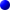
\includegraphics[width=0.5\textwidth]{./images/soma.pdf}
    \end{center}
    \caption{A soma with two dendrites.}
    \label{fig:soma}
\end{figure}

\fig{fig:soma} shows a soma that is attached to two unbranched dendrites.
In this example the simplest possible compartment model is used, with three compartments: one for the soma and one for each of the dendrites.
The soma CV extends to half way along each dendrite.
To calculate the flux from the soma compartment to the dendrites the flux over the CV face half way along each dendrite has to be computed.
For this we use the voltage defined at each end of the dendrite, which raises the question about what value to use for the end of the dendrite that is attached to the soma.
For this we use the voltage as defined for the soma, i.e. we use the same value at the start for each dendrite, as illustrated in \fig{fig:soma}.

This effectivly of ``collapses'' the node that defines the start of dendrites attached to the soma onto the soma in the mathematical formulation.
This requires a little slight of hand when loading the cell description from file (for example a \verb!.swc! file).
In such file formats there would be 5 points used to describe the cell in \fig{fig:soma}:
\begin{itemize}
    \item 1 to describe the center of the soma.
    \item 2 for each dendrite: 1 describing where the dendrite is attached to the soma, and 1 for the terminal end.
\end{itemize}
However, in the mathematical formulation there are only 3 values that are solved for: the soma and one for each of the dendrites.

On a side note, one possible extension is to model the soma as a set of shells, like an onion.
Conceptually this would look like an additional branch from the surface of the soma, with the central core being the terminal of the branch.
However, the cable equation would have to be reformulated in spherical coordinates.


%-------------------------------------------------------------------------------
\subsubsection{Handling Branches}
%-------------------------------------------------------------------------------
The value of the lateral area $\sigma_i$ in~\eq{eq:sigma_i} is the sum of the areaof each branch at branch points.

\todo{a picture of a branching point to illustrate}

\todo{a picture of a soma to illustrate the ball and stick model with a sphere for the soma and sticks for the dendrites branching off the soma.}

\begin{equation}
    \sigma_i = \sum_{j\in\mathcal{N}_i} {\dots}
\end{equation}

